\documentclass{standalone}
\usepackage{tikz}
\begin{document}
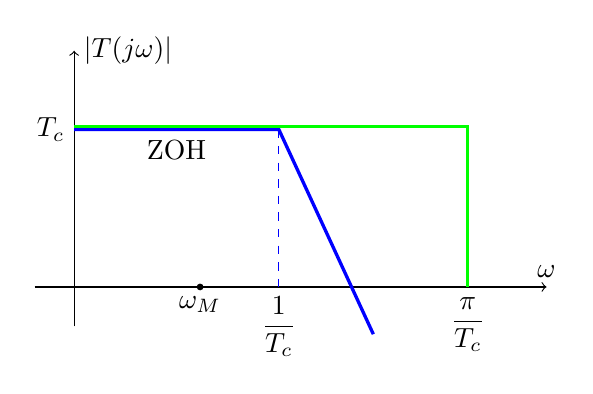
\begin{tikzpicture}[scale=2]
    \draw[->](-0.25,0)--(3,0)node[above]{$\omega$};
    \draw[->](0,-0.25)--(0,1.5)node[right]{$|T(j\omega)|$};

    \node[left]at(0,1){$T_c$};
    \draw[-,very thick,blue](0,1)--(1.3,1)node[black,midway, below]{ZOH}--(1.9,-0.3);
    \draw[dashed,blue](1.3,1)--(1.3,0)node[below, black]{$\displaystyle\frac{1}{T_c}$};
    \draw[-,very thick, green](0,1.02)--(2.5,1.02)--(2.5,0)node[below, black]{$\displaystyle\frac{\pi}{T_c}$};

    \filldraw[black](0.8,0)node[below]{$\omega_M$}circle(0.5pt);
\end{tikzpicture}
\end{document}